\documentclass[../notes.tex]{subfiles}

\begin{document}

\section{Introduction}

\subsection{Parallelism in the CPU}
\textbf{Basic five-stage RISC architecture}
\begin{itemize}
\item Instruction fetch (IF)
\item Instruction decode (ID)
\item Instruction execute (Ex)
\item Memory access (Mem)
\item Register write-back (WB)
\end{itemize}

\subsubsection{Pipelining (ILP, Instruction Level Parallelism)}
Process many instruction in one-clock cycle by diviing execution unit in multiple phases.
\begin{figure}[h]
  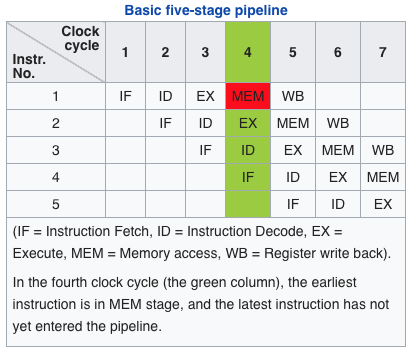
\includegraphics[width=6.2cm]{pipelining}
\end{figure}

\subsubsection{Superscalar}
Superscalar processor uses multiple execution units on the same chip to achieve ILP.
\begin{figure}[h]
  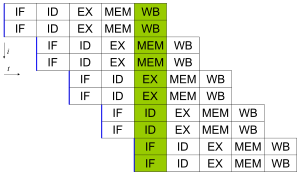
\includegraphics[width=6.2cm]{superscalar}
\end{figure}

\subsubsection{SMT Simultaneous Multithreading}
Take a few more CPI regisers, and execute more instructions on the part of the core that is sitting idle. Thus, one core now appears as two cores. But they are not completely independent. If both "cores" need to access the CPU resource, one of them end up waiting.

\subsection{Introduction to GPU}
CPUs prove to be inefficient to operate on large chunks of data. A GPU comprises many cores (that almost double each passing year), and each core runs at a clock speed significantly slower than a CPU's clock. GPUs focus on execution throughput of massively-parallel programs. When it comes to the total Floating Point Operations per Second (FLOPS), GPUs have been leading the race for a long time now.

{\color{blue} For example, RTX 2080 Ti has 4352 cores, with frequency from 1350 MHz to 1625 MHz, while Intel I9-9900k has only 8 cores, but with frequency from 3.6 GHZ to 5 GHZ.}

\begin{figure}[h]
  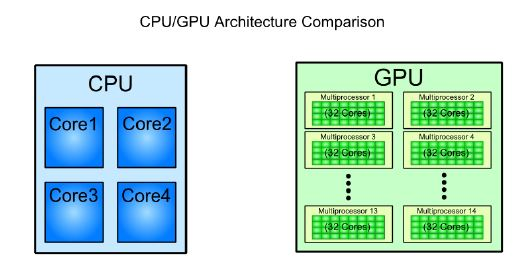
\includegraphics[width=12cm]{architecture_comparison}
\end{figure}

GPUs are designed for data intensive applications. They were originally designed for 3D rendering, which requires holding large amount of texture and polygon data.

\subsubsection{Memories}
\textbf{Different types of memories}
\begin{itemize}
  \item DRAM (Dynamic RAM) is the most common RAM found in systems today, and is also the slowest and the least expensive one. The RAM is named so because the information stored on it is lost, and the processor has to refresh it several times in a second to preserve data.
  \item SRAM (Static RAM) is significantly faster than DRAM (the difference in speeds comes from the design and the static nature of these RAMs). It is also called the microprocessor cache RAM. This cache is used by the processor to store frequently used data, so that for each request, it does not have to access the much slower DRAM.
  \item VRAM (Video RAM) is quite similar to DRAM but with one major difference: it can be written to and read from simultaneously. This property is essential for better video performance. Using it, the video card can read data from VRAM and send it to the screen without having to wait for the CPU to finish writing it into the global memory.
\end{itemize}

\newpage

\subsubsection{Fixed Functioning Graphics Pipelines}
The following image illustrates and describes a fixed-function Nvidia pipeline.
\begin{figure}[ht]
  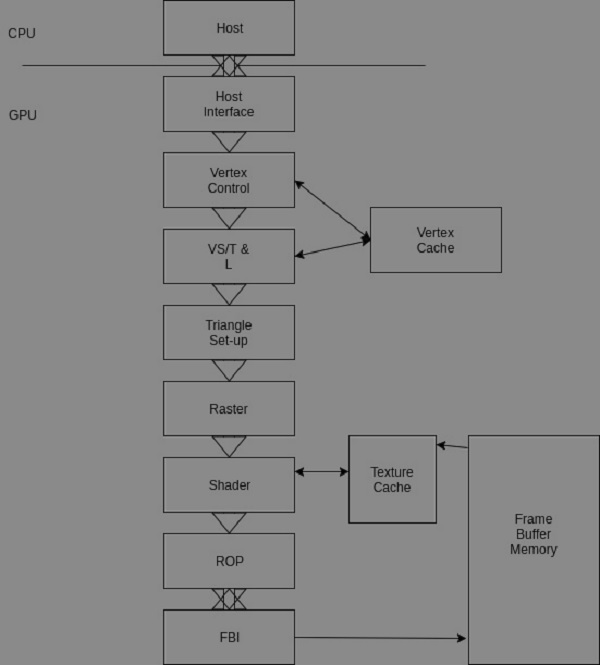
\includegraphics[width=10cm]{fixed_function_nvidia_pipeline}
\end{figure}

Let us understand the various stages of the pipeline now
\begin{itemize}
  \item The CPU sends commands and data to the GPU host interface. The commands are given by application programs by calling an API function.
  \item The vertex control stage receives parameterized triangle data from the host interface. Then it comes to VS/T\&L stage, which stands for Vertex Shading, Transform and Lighting. This stage transforms vertices and assigns each vertex values for some parameters, such as colors, texture coordinates, normals and tangents. The pixel shader hardware does the shading (the vertex shader assigns a color value to each vertex, but coloring is done later).
  \item The triangle setup stage is used to interpolate colors and other vertex parameters to those pixels that are touched by the triangle (the triangle setup stage actually determines the edge equations. It is the raster stage that interpolates).
  \item The shader stage gives the pixel its final color. There are many methods to achieve this, apart form interpolations. Some of them include texture mapping, per-pixel lighting, reflections, etc.
  \item The ROP stage (Raster Operation) is used to perform the final rasterization steps on pixels. For example, it blends the color of overlapping objects for transparency and anti-aliasing effects. It also determines what pixels are occluded in a scene (a pixel is occluded when it is hidden by some other pixel in the image). Occluded pixels are simply discarded.
  \item The FBI (Frame Buffer Interface) stage manages reading and writing from the display buffer memory.
\end{itemize}





\end{document}
